% ============================================================
%  cvstyle.tex -- shared preamble/macros for Zihao-Eric GUO's CV
%  Recreates the two-column "sidebar + timeline" Word template
%  used in CV_doc/*.docx (one page, A4).
%  Included by CV_Zihao_EN.tex / CV_Zihao_FR.tex / CV_Zihao_CH.tex
% ============================================================

\documentclass[10pt,a4paper]{article}

\usepackage[T1]{fontenc}
\usepackage[utf8]{inputenc}
\usepackage{carlito}                 % Calibri-metric-compatible font
\renewcommand{\familydefault}{\sfdefault}

\usepackage[paperwidth=210mm,paperheight=297mm,margin=0mm]{geometry}
\usepackage[absolute,overlay]{textpos}
\usepackage{eso-pic}
\usepackage{tikz}
\usetikzlibrary{shadows,shapes.geometric}
\usepackage{xcolor}
\usepackage{array}
\usepackage{ragged2e}
\usepackage{enumitem}
\usepackage{fontawesome5}
\usepackage{graphicx}
\usepackage[hidelinks]{hyperref}

\pagestyle{empty}
\setlength{\parindent}{0pt}
\renewcommand{\arraystretch}{1}

% ---------------- colours (sampled from the original docx) ----------------
\definecolor{cvblue}{HTML}{017BAA}   % banner / skill box / icon badges / bars
\definecolor{cvbluedark}{HTML}{004F6E}
\definecolor{cvgray}{HTML}{F3F3F3}   % sidebar + section-header bar
\definecolor{cvlink}{HTML}{0563C1}   % hyperlink blue
\definecolor{cvdot}{HTML}{0070C0}    % bullet / timeline rule blue
\definecolor{cvrule}{HTML}{BFBFBF}   % timeline grey rule
\definecolor{cvtext}{HTML}{000000}

\hypersetup{colorlinks=true, urlcolor=cvlink, linkcolor=cvlink}

% ---------------- text grid -------------------------------------------------
\setlength{\TPHorizModule}{1mm}
\setlength{\TPVertModule}{1mm}
\textblockorigin{0mm}{0mm}

% ---------------- layout dimensions -----------------------------------------
\newlength{\sidew}    \setlength{\sidew}{61mm}    % sidebar width
\newlength{\sidepad}  \setlength{\sidepad}{4mm}   % sidebar inner padding
\newlength{\mainx}    \setlength{\mainx}{64mm}    % right column x-origin
\newlength{\mainw}    \setlength{\mainw}{139mm}   % right column width

\newlength{\sideinnerw}
\setlength{\sideinnerw}{\sidew}
\addtolength{\sideinnerw}{-2\sidepad}

\newlength{\cvdatew}  \setlength{\cvdatew}{24mm}
\newlength{\cvgutter} \setlength{\cvgutter}{4mm}
\newlength{\cvcontw}
\setlength{\cvcontw}{\mainw}
\addtolength{\cvcontw}{-\cvdatew}
\addtolength{\cvcontw}{-\cvgutter}

% ---------------- full-bleed sidebar background -----------------------------
\AddToShipoutPictureBG*{%
  
\begin{tikzpicture}[remember picture,overlay,x=1mm,y=-1mm]
    \fill[cvgray] (0,0) rectangle (61,297);
  \end{tikzpicture}%
}

% ---------------- generic helpers -------------------------------------------

% small filled dot bullet (sidebar contact rows / language rows)
\newcommand{\cvdotmark}{\textcolor{cvdot}{\Large\textbullet}}

% language proficiency bar: #1 = fill fraction in [0,1]
\newcommand{\langbar}[1]{%
  \begin{tikzpicture}[x=1mm,y=1mm]
    \def\w{45}\def\h{3.2}
    \draw[black, line width=0.6pt, rounded corners=0.7pt] (0,0) rectangle (\w,\h);
    \fill[cvblue] (0.18,0.18) rectangle ({#1*\w-0.18},{\h-0.18});
  \end{tikzpicture}%
}

% sidebar section title (bold black, no bar)
\newcommand{\sidetitle}[1]{%
  \par\vspace{1mm}\textbf{\Large #1}\par\vspace{1.3mm}%
}

% compact sidebar education entry: #1=institution #2=dates/location #3=description
\newcommand{\sideedu}[3]{%
  \cvdotmark\ \textbf{\normalsize #1}\par\vspace{0.6mm}
  {\footnotesize\textit{\textcolor{black!65}{#2}}}\par\vspace{0.6mm}
  {\footnotesize\itshape #3}\par%
}

% section badge + heading bar for the main column
% #1 = fontawesome icon command   #2 = heading text
\newcommand{\cvsection}[2]{%
  \par\vspace{6mm}\noindent%
  \begin{tikzpicture}[baseline=-3.2mm,x=1mm,y=1mm]
    \node[fill=cvblue, rounded corners=1.2pt, minimum width=8mm, minimum height=8mm, inner sep=0pt]
      (badge) at (4,-4) {\textcolor{white}{\fontsize{11}{11}\selectfont #1}};
    \fill[cvblue] (1.2,-7.6) -- (3,-8.6) -- (3,-7.6) -- cycle; % small tail
  \end{tikzpicture}%
  \hspace{1.5mm}%
  \colorbox{cvgray}{\makebox[127mm][l]{\rule{0pt}{3.6mm}\textbf{\Large \MakeUppercase{#2}}}}%
  \par\vspace{2.8mm}%
}

% timeline row: #1=date (bold)  #2=location (italic)  #3=main content
\newcommand{\cvrow}[3]{%
  \noindent
  \begin{tabular}{@{}p{\cvdatew}!{\color{cvrule}\vrule width 0.8pt}p{\cvcontw}@{}}
  \begin{minipage}[t]{\cvdatew}\raggedright\textbf{#1}\par\vspace{0.8mm}\textit{\textcolor{black!65}{#2}}\end{minipage}
  & \hspace{3mm}\begin{minipage}[t]{\cvcontw}#3\end{minipage}\\
  \end{tabular}\par\vspace{6mm}%
}

% continuation row (no date/location repeated, just the rule + content)
\newcommand{\cvcont}[1]{%
  \noindent
  \begin{tabular}{@{}p{\cvdatew}!{\color{cvrule}\vrule width 0.8pt}p{\cvcontw}@{}}
  \mbox{} & \hspace{3mm}\begin{minipage}[t]{\cvcontw}#1\end{minipage}\\
  \end{tabular}\par%
}

\newcommand{\kw}[1]{\underline{\texttt{\footnotesize #1}}}

\newcommand{\entrydate}[1]{\hspace{3mm plus 1fill}\textit{\underline{#1}}}

\newlist{cvitemize}{itemize}{1}
\setlist[cvitemize]{leftmargin=4mm, itemsep=0pt, topsep=1pt, parsep=0pt, label=\textbullet}

\newlist{sideitemize}{itemize}{1}
\setlist[sideitemize]{leftmargin=3mm, itemsep=0.5pt, topsep=1pt, parsep=0pt, label=\textbullet}


\begin{document}

% =========================== SIDEBAR (left) ===========================
\begin{textblock*}{\sideinnerw}(\sidepad,6mm)
\begin{minipage}[t]{\sideinnerw}
\begin{tikzpicture}
  \clip (0,0) circle (16mm);
  \node[anchor=center] at (0,0) {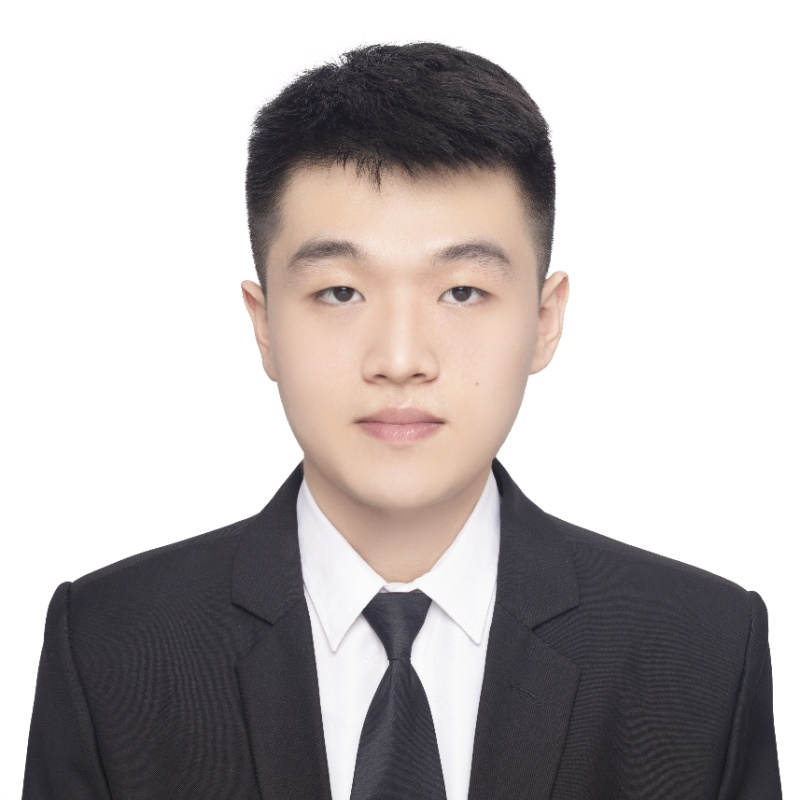
\includegraphics[width=34mm]{assets/photo.jpg}};
\end{tikzpicture}

\vspace{4mm}
{\LARGE\textbf{Zihao-Eric GUO}}\par
\vspace{3.5mm}

{\normalsize
\faEnvelope\ \href{mailto:zihao-eric.guo@ip-paris.fr}{zihao-eric.guo@ip-paris.fr}\par\vspace{1.8mm}
\faPhone\ +33 (0)765241550\par\vspace{1.8mm}
\faMapMarker\ Paris, France\par\vspace{1.8mm}
\faKaggle\ Kaggle Expert\par\vspace{1.8mm}
\faHome\ \href{https://zihao-guo.github.io/}{Welcome to my homepage}\par
}

\vspace{2mm}
\sidetitle{EDUCATION}
\sideedu{Institut Polytechnique de Paris}{Since 11/2023 -- Paris, France}{Preserving graph performance in an exogenously perturbed environment - Expected graduation date: \textbf{\underline{Dec.2026}}}
\vspace{2mm}
\sideedu{École Centrale de Nantes}{09/2021 -- 09/2023 -- Nantes, France}{Generalist Engineer Degree - Applied Mathematics Options}
\vspace{2mm}
\sideedu{Université de Picardie Jules Verne}{09/2017 -- 07/2021 -- Amiens, France}{Bachelor of Science, Optimization}

\vspace{2mm}
\sidetitle{IT SKILLS}
\tikz\node[fill=cvblue, text=white, rounded corners=2pt, text width=\sideinnerw-4mm, inner sep=2.2mm]{\normalsize Python (NumPy, Pandas, Sklearn, PyTorch, Plotly), R, C/C++, NoSQL, MATLAB, Power BI, Catia, CAD};

\vspace{2mm}
{\small\itshape\justifying Hilbertian analysis, Stochastic Process, statistical learning, Bayesian methods and hierarchical models, Probabilistic numerical methods, Databases, Uncertainty Quantification, Algorithms \& Programming, Physics and Fluid Dynamics, Data Science \& Machine Learning, Optimization, Signal and Systems, Finite Elements.\par}

\vspace{2mm}
\sidetitle{LANGUAGES}
{\normalsize
\cvdotmark\ \textbf{Chinese}: Native language\par\vspace{1mm}
\langbar{0.95}\par\vspace{2mm}
\cvdotmark\ \textbf{English}: Fluent (GRE 326)\par\vspace{1mm}
\langbar{0.82}\par\vspace{2mm}
\cvdotmark\ \textbf{French}: Fluent (DALF C1)\par\vspace{1mm}
\langbar{0.72}\par
}

\vspace{2mm}
\sidetitle{INTERESTS}
\textcolor{cvblue}{\LARGE\faBookOpen\ \faBasketballBall\ \faFutbol\ \faKeyboard}\par

\vspace{2mm}
\sidetitle{Aces}
{\normalsize\itshape
\begin{sideitemize}
\item Team spirit;
\item independence and adaptability;
\item High learning capacity.
\end{sideitemize}
}
\end{minipage}
\end{textblock*}

% =========================== MAIN COLUMN (right) ===========================
\begin{textblock*}{\mainw}(\mainx,6mm)

% ---- banner ----

\begin{tikzpicture}[x=1mm,y=-1mm]
  \node[fill=black!15, rounded corners=3pt, minimum width=139mm, minimum height=27mm, inner sep=0pt] at (70.7,14.8) {};
  \shade[shading=axis, left color=cvblue, right color=cvbluedark, shading angle=-25,
        rounded corners=3pt] (0,0) rectangle (139,27);
  \node[anchor=north west, text=white, text width=95mm, align=left, inner sep=0pt] at (5,4)
    {\faIdBadge\ Pre-Doc @ Institut Polytechnique de Paris\par\vspace{0.8mm}Interested in: Stochastic Optimization, Math Programming};
  \node[anchor=north east, text=white] at (134,19.5)
    {\large\textbf{AI Engineer | Algorithm Engineer | Data Scientist}};
  \node[fill=white, minimum width=8mm, minimum height=8mm, inner sep=0pt] at (113,7) {\href{https://www.linkedin.com/in/zihao-éric-g-850167211/}{\textcolor{cvblue}{\large\faLinkedin}}};
  \node[fill=white, minimum width=8mm, minimum height=8mm, inner sep=0pt] at (124,7) {\href{https://github.com/zeio99}{\textcolor{black}{\large\faGithub}}};
\end{tikzpicture}
\vspace{-1mm}

% ---- INDUSTRIAL EXPERIENCE ----
\cvsection{\faFlag}{Industrial Experience}

\cvrow{2025}{Shanghai,\\ \textbf{\itshape CHINA}}{%
\textbf{Internship -- Algorithm Engineer (\href{https://www.huawei.com/fr/}{Huawei})}\entrydate{08/2025 -- 11/2025}\par
{\normalsize\begin{cvitemize}
\item Developed a point cloud--channel multimodal contrastive learning framework for accurate channel prediction and proposed an integer-partitioning-based non-contiguous resource allocation algorithm improving RIV continuous allocation.
\end{cvitemize}
Keywords: \kw{Multimodal contrastive learning, Optimization}}}

\cvrow{2023}{Cambridge,\\ \textbf{\itshape UK}}{%
\textbf{Internship -- Biostatistics Researcher Intern (\href{https://en.wikipedia.org/wiki/European_Bioinformatics_Institute}{EMBL-EBI})}\entrydate{04/2023 -- 09/2023}\par
{\normalsize\begin{cvitemize}
\item The research topic is ``Simulating the evolution of genomes along large, short-branch phylogenetic trees''
\end{cvitemize}
Keywords: \kw{R/Python, Sampling algorithm, Cluster, bash(UNIX)}}}

\cvrow{2022}{Paris,\\ \textbf{\itshape France}}{%
\textbf{Internship -- Data Engineer (\href{https://www.ifpenergiesnouvelles.com/}{IFPEN})}\entrydate{04/2022 -- 08/2022}\par
{\normalsize\begin{cvitemize}
\item Analysis of traffic badge validation data and create a dashboard.
\item Comparison of data obtained from a traffic model (MATSim) to explore errors.
\item Using time series models (Sarimax, Neuralprophet...) to analyze the impact of influencing factors and correct the statistics by predicting the data.
\end{cvitemize}
Keywords: \kw{Django, HTML/CSS, MongoDB, Git, Pytorch, Statsmodels}}}

% ---- SCIENTIFIC RESEARCH EXPERIENCE ----
\cvsection{\faTrophy}{Scientific Research Experience}

\cvrow{}{}{%
\textbf{LLM-related Research}\entrydate{Since 2025}\par
{\normalsize\begin{cvitemize}
\item Developed \textbf{EvoHGS}, an LLM-guided framework for improving Hybrid Genetic Search on vehicle routing problems through solver-in-the-loop optimization.
\item Followed and customized the MiniMind pipeline to practice the full lightweight LLM workflow.
\end{cvitemize}
Keywords: \kw{C++, Supervised Fine-Tuning, LoRA, GRPO}}}

\cvrow{Oct.22 - Apr.23}{Nantes, France}{%
\textbf{Research - Multi-task learning for Bayesian Networks}\entrydate{Nantes Digital Science Laboratory (LS2N)}\par
{\normalsize Keywords: \kw{C++, Linux, Bayesian Networks, Transfer learning}}\par
\textbf{Research - Extreme value theory with environmental applications}\entrydate{École Centrale de Nantes (ECN)}\par
{\normalsize Keywords: \kw{Statistical Modeling}}}

\cvcont{%
\textbf{Essay - CNN text classification method based on simulated annealing method}\entrydate{\textit{ACM - International Conference Proceeding Series (ISBN: 978-1-4503-8432-2)}}\par
\textbf{Essay - Restoring Accessibility During Urban Rail Disruptions via Bus Network Redesign}\entrydate{\textit{Transportation Research Board (TRB) 104th Annual Meeting}}\par
\textbf{Essay - Rate variation and recurrent sequence errors in pandemic-scale phylogenetics}\entrydate{\textit{Nature Methods}}\par
\vspace{1.5mm}
\centerline{\small For more publications, please visit my \href{https://scholar.google.com/citations?view_op=list_works&hl=en&hl=en&user=gMy-9XEAAAAJ}{Google Scholar profile}.}}

\end{textblock*}

\end{document}
